\section{REQUIREMENT ANALYSIS AND DESIGN}\label{sec:design-decision}

\subsection{Gathering user requirements and specifications.}\label{subsec:Gathering user requirements and specifications.}
To develop a system that fulfilled the user requirements, it was important for us to understand who could be the users of our system. Some of the primary users we identified are: Internet measurements researchers, internet traffic engineering practitioners and ISPs routing administrators. After identifying the users, we decided to speak to the users to get some of their desired use cases. One of the user we identified was our supervisor who is an internet measurement researcher and traffic engineer. His experience in the internet measurements field made him a suitable user to speak to about the system and gather requirements that could be expected. The other users we spoke to are postgraduates students who are pursuing network studies as their knowledge in networks could help them identify efficient use cases they may be interested to perform with system.

\subsubsection{Regular meetings with the supervisor}
 The first three meetings with the supervisor involved in- depth discussion on the goals of the project. We ensured that everyone in the team had understood the project before the development had started. Throughout the project timeline, we held progress meetings with the supervisor to ensure that the project and the platform was being developed in accordance with user requirements.  These meetings gave us confidence that we were developing a system that was useful. Any challenge that was encountered during the development could be addressed during the meetings or through follow up emails with the supervisor.  
\subsubsection{Observations}
A related capstone project that was focusing on creating an inter-domain simulator had been done in 2019. We therefore decided to contact group members who had done the project and requested them to demo to us so that we could see what they had done. The group members agreed and we observed the features that had been implemented. Afterwards, we confirmed with our client so that we could implement some of those features in our system.
\subsubsection{Prototyping}
To demonstrate to the user whether we had captured the right user requirements, we developed a project prototype within two weeks which we demoed to the user. The prototype was evolutionary and horizontal as we wanted to first focus on how the user will interact with whole system and keep adding more features to the prototype based on the user feedback after the demo. During the demo, the user gave feedback that the geographical map that the visualizer and the simulator were using needed to implement layering. This feedback was important as we managed to get that layering was a user requirement. We also explained to the user the set of features that were to be implemented after the demo which were to check whether the features were relevant in fulfilling user requirements.   
\subsubsection{Gathered user requirements}
After collecting the user requirements, we analysed them and grouped them into both functional and nonfunctional requirements. Functional requirements are the requirements we gathered that defined some of the functions the system needed to achieve while non-functional requirements are the attributes that defined some of the factors that could be used to determine how good the system was. 

The functional requirements we collected for the simulator includes: allow the user to add an IXP node to the topology, allow the user to delete a node from the topology, allow the user to add a connection between two nodes, allow the user to delete a connection between two nodes and enable the user to view the routing path of the simulated internet traffic and the link delay of the routing path. These requirements are to enable the user to manipulate the internet topology to evaluate how each action could affect the internet performance hence they formed the functional requirements of the simulator. 


The non-functional requirements we collected for the simulator includes: The simulator should be hosted online and everyone who wishes to use it should access it freely. That is, the simulator should not require the user to do prior installation. Hosting it online was necessary as we expected to do remote user testing due to limitations that we could not do face to face testing. The simulator should also be easier to use and have a good user interface to ensure the user could use the simulator effectively without depending on guidance from the development team. The simulator should be reliable and free from software bugs so as to guarantee a good user experience. The simulator should be able to run effectively and faster even when being by many concurrent users. 



\subsection{System Design}
After collecting and analysing the user requirements, we decided to design our system by looking at how the requirements were related to each other by designing the use case diagram. To visualize how various subsystems will interact with each other, we decided to design the package diagrams to show at high level how various subsystems would relate to each other. Topology is the primary component that responds to change of events during simulation and due to this, we decided to design a state machine diagram to illustrate how the internet topology responded to various changes that happened during simulation. 
\subsubsection{Use case diagram}
To summarize the functional requirements in a visual design diagram, use-case diagram was designed as shown in Figure 1. The use-case diagram was important as it represented the goals that can be achieved from the user-system interactions. The use-case diagram also communicated how various use cases were related either through the "extend" relationship or "include" relationship.

The "Add IXP node" use case has an include relationship with "Delete IXP node" since you cannot delete an IXP node that has not been already added in the topology. The "Simulate Traffic Flow" use case has an include relationship with "View RTT" use case since it through simulating traffic flow that RTT can be determined and viewed. The "Remove a connection" use case has an extend relationship with "Add a connection" since some connections are added to the topology during the pre-simulation phase of the system.

\begin{figure}[htp]
   \centering
     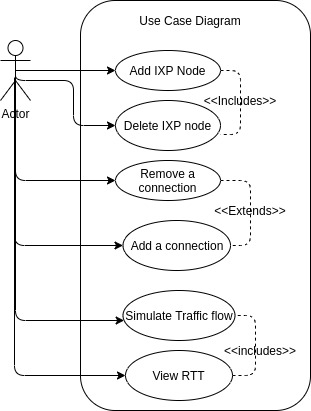
\includegraphics[width=8.5cm]{sections/pictures-diagrams/usecasedigarma.jpg}
   \caption{Use case diagram for the system.}
    \label{figure:galaxy}
\end{figure}

\subsubsection{Package diagram}
\begin{figure}[htp]
   \centering
     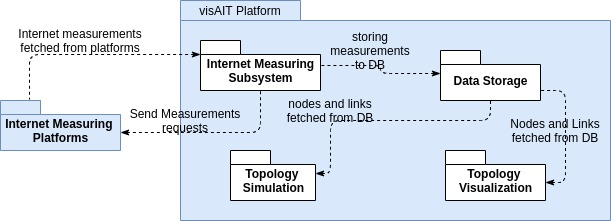
\includegraphics[width=10cm]{sections/pictures-diagrams/Package-Diagrma-v2.jpg}
   \caption{Package diagram showing various subsystems of the platform.}
    \label{figure:galaxy}
\end{figure}
The package diagram is used to show subsystems of a system on a high level. The package diagram we designed is illustrated in Figure 2 and it was used to visualize how various subsystems of the platform will depend and interact with each other. The diagram also showed how the system will look like in a more modular manner. 

The topology simulation subsystem depends on other three subsystems namely: Internet measuring subsystem,  topology visualization subsystem and Data Storage. Internet measuring platforms is an external package since the internet measuring platforms runs independently from our system. our system only interacts with the internet measuring platforms via API calls when measurements requests are sent by the internet measuring subsystem. The data storage subsystem stores data that has been collected by the internet measuring subsystem. The topology simulation and topology visualization subsystems interacts with the data storage to access the links and nodes' information that is stored in the data storage. 

\subsubsection {State Machine diagram}
State machine diagram illustrated in Figure 3 shows the various states the internet topology may be during simulation. The diagram shows how the topology transitions from one state to another when an event happens.

During pre-simulation phase, the topology is in idle state. When an node is removed from topology, the remove node method is invoked and the topology will transition to the state where the topology is shown without the removed node. When an IXP node is added to the topology, the add IXP node method is invoked and the topology transition to the state where the topology is shown with the added node. When a connection between two nodes is added to the topology, the add connection method is invoked and the topology transition to the state where the topology is shown with the added connection. When a connection between two nodes is removed from the topology, the remove connection method is invoked and the topology transition to the state where the topology is shown without the removed connection.

At any given state, the simulate traffic method can be invoked and the topology will transition to the state where the routing route and the link delay is shown. This was important as any action done on the internet topology could be evaluated of its effect on internet performance. 
\begin{figure*}
    \begin{center}
        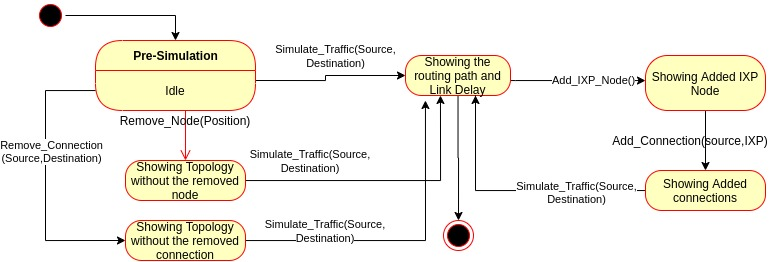
\includegraphics[width=1\linewidth]{sections/pictures-diagrams/sequence.jpg}
    \end{center}
    \caption{Diagram showing various states the topology may be during simulation}
    \label{figure:state}
\end{figure*}
\subsubsection{Link Delay and Routing Algorithm design}
Link delay is the metric used to determine performance of the scenario being tested during simulation is. Since every link is associated with link delay, the challenge was how to assign link delay to the new introduced links. According to Günther \textit{et al}\cite{RTTT}, the minimum Round Trip Time(RTT) internet traffic takes from a source to destination can be computed as: 
\begin{equation}
RTT(min) = 2*d/c
\end{equation}
\textit{where d is the distance 
between the source and the destination and c is the speed of light which is: }
\begin{equation}
c = 3*10^8
\end{equation}

We adopted this method to assign the link delays of the newly introduced connections during simulation. 

To determine the best route of internet traffic from source to destination, we implemented the Dijkstra's algorithm\cite{SaeediMEJ10} to determine the shortest distance between the source and the destination.  